\documentclass[]{report}

\voffset=-1.5cm
\oddsidemargin=0.0cm
\textwidth = 480pt

\usepackage{framed}
\usepackage{subfiles}
\usepackage{graphics}
\usepackage{newlfont}
\usepackage{eurosym}
\usepackage{amsmath,amsthm,amsfonts}
\usepackage{amsmath}
\usepackage{color}
\usepackage{amssymb}
\usepackage{multicol}
\usepackage[dvipsnames]{xcolor}
\usepackage{graphicx}
\begin{document}

\section{Correlation}
\begin{itemize}
	\item Correlation is a measure of the relation between two or more variables. 
	%\item The measurement scales used should be at least interval scales, but other correlation coefficients are available to handle other types of data.
	\item Correlation coefficients can range from -1.00 to +1.00. The value of -1.00 represents a perfect negative correlation while a value of +1.00 represents a perfect positive correlation. A value of 0.00 represents a lack of correlation.


	\item 
	The most widely-used type of correlation coefficient is Pearson r, also called linear or product- moment correlation.
	The pearson correlation coefficient is a metric.

	\item  Two variables that have no linear relationship have a correlation close to zero. 
	
	\item Scatter plots are a useful way of determing the likely relationship between two variables. 
	
	\item The Pearson correlation coefficient is most commonly used estimate for correlation. 
	
	\item Other types of correlation are tbe \textit{\textbf{Spearman Rho}} and the \textit{\textbf{Kendal Tau}} correlation coefficients. 
	
	%\item  These are not not part of this course,but it is important to know that they exist. 
\end{itemize}
%--------------------------------------------- %



\begin{itemize}
	\item Correlation is a measure of strength of \textbf{Linear Relationship} between two variables.
	\item The Pearson correlation coefficient (denoted $r$) is the most comonly used statistical estimate for correlation. 
	\item Correlation estimates are defined to be between -1 and 1. It is not possible to have a correlation value outside this range of values
	\[ -1 \leq r \leq 1\]
	\item 
	Additionally correlation estimates are not denominated in any units. (Contrast this to standard deviation, which is denominated in the same units as the mean).
\end{itemize}

%--------------------------------------------- %



\begin{itemize}
	\item A strong positive linear relationship describes a relationship between two variables whereby an increase in one variable will closely coincide with an increase in the other variable. 
	\item Conversely a strong negative linear relationship describes a relationship whereby an increase in one variable closely coincides with a decrease in the other. 
\end{itemize}
\begin{itemize}
	\item The Pearson correlation estimate, which us based on sample data, is denoted r (although related metrics use capital R).
	\item This measure is used as an estimate for the Population correlation, denoted by the greek letter $\rho$ ( pronounced ``Rho"). 
	The estimate is computed using summation identities.
	% (See the formulae ).
	
	%\item 
	%Equivalently it can be computed using the  Sums of Squares Identities that are used to compute covariance and standard deviation <INSERT FORMULA> .
	%Example
	%determine the correlation estimate for the Spend V Impressions data.  
\end{itemize}
%-------------------------------------------------------- %


\subsection{Outliers}
\begin{itemize}
	\item Outliers can greatly influence the computed value of an estimate.
	\item  Correlation is closely related to Simple linear regression models, in that both are concerned with the linear relationship between variables. However Linear Regression has a different emphasis.
	\item  Simple Linear Regression describes one independent variable (IV) and the response of the dependent variable (DV). 
\end{itemize}





\subsection{Correlation and Causality }
Implicit is simple linear regression is the notion of causality. The dependent variable changes as the independent variable changes. The converse is not true.
<some examples : hot temperature / ice cream example> .
Correlation is not concerned with causality at all, hence the often used expression "causation does not imply causality ".

%-----------------------------------------------------%

%---------------------------------------------------------------------%

\section{Correlation}
\begin{itemize}
	\item This is a measure of Strength of Linear Relationship.
	The correlation estimate is defined to be between -1 and 1.
	\item It is not possible to have a correlation value outside this range of values
	Additionally correlation estimates are not denominated in any units. (Contrast this to standard deviation, which is denominated in the same units as the mean ) .
	\item A strong positive linear relationship describes a relationship between two variables whereby an increase in one variable will closely coincide with an increase in the other variable.
	\item Conversely a strong negative linear relationship describes a relationship whereby an increase in one variable closely coincides with a decrease in the other.
\end{itemize}


\subsection{Correlation and cause-effect}
\begin{itemize}
	\item Note that a strong relationship between two variables does not
	imply a cause-effect relationship.
	\item For example, there is a strong negative correlation between the
	sales of ice cream and the number of flu infections.
	\item This does not mean that ice cream protects against flu.
	\item This relationship results from a latent variable (a variable that has
	not been observed).
	\item Such a latent variable in this case is the weather. Low
	temperatures and wet weather result in a high number of flu
	infections and low ice cream sales. \item Hot, sunny weather leads to the
	opposite.
\end{itemize}



%---------------------------------------------------------------------%

\subsection{Correlation Coefficient : Formula}
The estimate of the Pearson correlation coefficient is given by
\[ r_{XY} = \frac{S_{XY}}{\sqrt{S_{XX}S_{YY}}} \]





%-------------------------------------------------%
\section{Correlation Coefficient}
\begin{itemize}
\item The Pearson correlation coefficient is a way of measuring the
strength of the relationship between two quantitative variables.

\item A correlation coefficient is a number between -1 and 1 which measures the degree to which two variables are linearly related. 
\item If there is perfect linear relationship with positive slope between the two variables, we have a correlation coefficient of 1; if there is positive correlation, whenever one variable has a high (low) value, so does the other. 
\item If there is a perfect linear relationship with negative slope between the two variables, we have a correlation coefficient of -1; if there is negative correlation, whenever one variable has a high (low) value, the other has a low (high) value. A correlation coefficient of 0 means that there is no linear relationship between the variables.
\item 
There are a number of different correlation coefficients that might be appropriate depending on the kinds of variables being studied.
\end{itemize}



%---------------------------------------------------------------------%

%========================================================================%

\subsection*{Correlation}
\begin{itemize}
	\item Recall that correlation describes the strength of a relationship between two numeric variables, and that the \textbf{\textit{Pearson product-moment correlation coefficient}} is a measure of the strength of the linear relationship between two variables.
	
	\item It is referred to as \textbf{Pearson's correlation} or simply as the correlation coefficient. If the relationship between the variables is not linear, then the correlation coefficient does not adequately represent the strength of the relationship between the variables.
	
	\item The symbol for Pearson's correlation is ``$\rho$" when it is measured in the population and \texttt{\textbf{r}} when it is measured for a sample.
	
	\item As we will be dealing almost exclusively with samples, we will use \texttt{\textbf{r}} to to represent Pearson's correlation unless otherwise noted.
	
	\item Pearson's r can range from -1 to 1. An estimate of -1 indicates a perfect negative linear relationship between variables, an \texttt{\textbf{r}} of 0 indicates no linear relationship between variables, and an \texttt{\textbf{r}} of 1 indicates a perfect positive relationship between variables.
	
	\item Importantly it is assumed that the relationship in question is supposed to be linear. Some variables will in fact have a non-linear relationship (more on that later)
\end{itemize}

\section{Pearson's Product Moment Correlation Coefficient}
\begin{itemize}
\item Pearson's product moment correlation coefficient, usually denoted by r, is one example of a correlation coefficient. It is a measure of the linear association between two variables that have been measured on interval or ratio scales, such as the relationship between height in inches and weight in pounds. 
\item 
However, it can be misleadingly small when there is a relationship between the variables but it is a non-linear one.
\item The Pearson correlation coefficient is only appropriate for
	describing the relationship between two quantitative variables
	which have a linear or near linear relationship

\item
There are procedures, based on r, for making inferences about the population correlation coefficient. 
\item However, these make the implicit assumption that the two variables are jointly normally distributed. 
When this assumption is not justified, a non-parametric measure such as the Spearman Rank Correlation Coefficient might be more appropriate.
\end{itemize}

%---------------------------------------------------------------------%
\begin{framed}
\subsection{Pearson's Correlation Coefficient.}

The Pearson correlation coefficient is a way of measuring the
strength of the relationship between two quantitative variables.

\begin{itemize}
	\item The population correlation coefficient between two variables X and
	Y is denoted by $\rho_{X,Y}$ .
	\item Used as an estimate for true correlation $\rho$.
	\item The population correlation coefficient between two variables X and
	Y is denoted by $\rho_{X,Y}$ .
	\item Used as an estimate for true correlation $\rho$.
	\item Pearson's Coefficient is denoted $r$.
	\item The Pearson Coefficient is defined to be between -1 and 1.
	\item The Pearson correlation coefficient is only appropriate for
	describing the relationship between two quantitative variables
	which have a linear or near linear relationship

	\item The Pearson Coefficient is defined to be between -1 and 1.

\end{itemize}

The Pearson Coefficient is computed using the following formula.
\[ r = \frac{S_{xy}}{(S_x)(S_y)} \]

\end{framed}
\subsection{Other Correlation Coefficients}
Pearson's Correlation Coefficient is one approach to estimating the strength of relation between two variables.
Other approaches are as follows:
\begin{itemize}
	\item Spearman's Rank Correlation
	\item Kendall Tau Correlation
\end{itemize}
These are not part of the course.



%---------------------------------------------------------------------%

%---------------------------------------------------------------------%

\subsection{Properties of the Correlation Coefficient}
\begin{enumerate}
	\item $-1 \leq r \leq +1$
	\item r = +1 or -1 represents a perfect linear correlation or a perfect linear
	relationship between the variables.
	\item r = 0 indicates little or no relationship i.e. as X increases there is no
	definite tendency for the value of Y to increase or decrease in a straight line.
	\item r close to +1 indicates a large positive correlation i.e. Y tends to increase
	as X increases.
	\item r close to -1 indicates a large negative correlation i.e. Y tends to decrease
	as X increases.
	\item The more r differs from 0, the stronger the linear relationship between the
	two variables.
	\item The sign of r indicates the direction of the relationship.
\end{enumerate}
%---------------------------------------------------------------------%


\section{Correlation and Regression}
Correlation
The Pearson's Product Moment Correlation Coefficient tells us how well two sets of continuous data correlate to each other. The value can fall between 0.00 (no correlation) and 1.00 (perfect correlation). A p value tells us if the Pearson's is significant or not. Generally p values under 0.05 are considered significant.

\subsection{Example 1}
%============================================================%

The height of a boy was observed at 7 different ages.
Comment on the relationship between height and age over this
period of time and calculate the Pearson correlation coefficient for
this data.
\begin{figure}
	% Requires \usepackage{graphicx}
	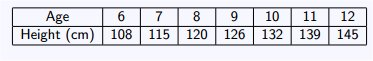
\includegraphics[scale=0.6]{images/11Bdata.jpg}\\
	
\end{figure}
\begin{itemize}
	\item X (the predictor variable) is defined to be age a
	\item Y is defined
	to be height (the dependent variable).
\end{itemize}


%Age  & 6 & 7  & 8 & 9 & 10 & 11 & 12 \\ 
%Height (cm)& 108 115& 120 &126& 132& 139 & 145\\

In order to investigate the nature of the relationship, we draw a
scatter plot.
X (the independent variable) is defined to be age and Y is defined
to be height (the dependent variable).


% http://www.statstutor.ac.uk/resources/uploaded/spearmans.pdf


\section{Correlation}

This requires a simple calculation based in values given and the relevant formula.

The formula for the Correlation estimate is as follows.

The calculated value should be between -1 and 1.

The following conclusions are drawn , depending on the Correlation estimate value:
\begin{itemize}
	\item Greater than 0.9 		Very strong positive linear relationship 
	\item Between 0.7 and 0.9		Strong positive linear relationship 
	\item Between 0.2 and 0.7	 	Weak positive linear relationship
	\item Between -0.2 and 0.2		No relationship
	\item Between -0.7 and -0.2		Weak negative linear relationship
	\item Between -0.9 and -0.7		Strong negative linear relationship
	\item Less than -0.9			Very strong negative linear relationship
\end{itemize}
Your answer should concur with your interpretation of the scatterplot.


Part 2 Correlation
This requires a simple calculation based in values given and the relevant formula.






Strength of a linear relationship between $X$ and $Y$

\begin{framed}
	\begin{verbatim}
	M=1000
	CorrData=numeric(M)
	for (i in 1:M)
	{
	CorrData[i] = cor(rnorm(10),rnorm(10))
	}
	\end{verbatim}
\end{framed}




%---------------------------------------------------------------------%

{Correlation Coefficient : Summations}
\begin{centering}
\begin{figure}
  % Requires \usepackage{graphicx}
  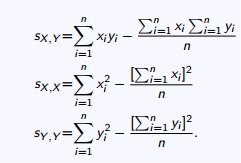
\includegraphics[scale=0.7]{images/11Bpearson.jpg}\\
  \caption{Summations}\label{11bpear}
\end{figure}
\end{centering}
%---------------------------------------------------------------------%






\begin{figure}
  % Requires \usepackage{graphicx}
  \includegraphics[scale=0.7]{images/11BPlot1.jpg}\\

\end{figure}
$r_{xy} = 0.87$ Strong Positive Linear Relationship




\begin{figure}
  % Requires \usepackage{graphicx}
  \includegraphics[scale=0.7]{images/11BPlot2.jpg}\\

\end{figure}

$r_{xy} = -0.258$ (Almost) No Relationship



\begin{figure}
  % Requires \usepackage{graphicx}
  \includegraphics[scale=0.7]{images/11BPlot3.jpg}\\

\end{figure}

$r_{xy} = -0.954$ Strong, though clearly non-linear




\begin{figure}
  % Requires \usepackage{graphicx}
  \includegraphics[scale=0.7]{images/11BPlot4.jpg}\\

\end{figure}
$r_{xy} =  -0.051$ (although there is a very strong
relationship)


%{Outliers}
%Outliers can greatly influence the computed value of an estimate.
%Correlation is closely related to Simple linear regression models, in that both are concerned with the linear relationship between variables. However Linear Regression has a different emphasis.
%Simple Linear Regression describes one independent variable (IV) and the response of the dependent variable (DV).
%




{Pearson's Product Moment Correlation Coefficient}
\begin{itemize}
\item Pearson's product moment correlation coefficient, usually denoted by r, is just one example of a correlation coefficient.
\smallskip
\item However, these make the implicit assumption that the two variables are jointly normally distributed. \smallskip
\item 
When this assumption is not justified, a non-parametric measure such as the Spearman Rank Correlation Coefficient might be more appropriate.
\end{itemize}




%---------------------------------------------------------------------%
%---------------------------------------------------------------------%

\subsection{Properties of the Correlation Coefficient}
Example: We are given data for 6 graduates. Below is their
final QCA and their corresponding starting salary after
graduation.
\begin{tabular}{|c|c|c|c|c|c|c|}
  \hline
 Subject & 1 &2 &3 &4 &5 &6\\
 Final QCA &2.8& 3.4& 3.2& 3.8& 3.2& 3.4\\
 Starting Salary &20 000 &24 500& 23 000& 25 000 &20 000 &22 500\\
  \hline
\end{tabular}


\begin{itemize}
\item Calculate the sample correlation coefficient.
\end{itemize}



%---------------------------------------------------------------------%

{Regression}
A statistical measure that attempts to determine the strength of the relationship between one dependent variable
(usually denoted by Y) and a series of other changing variables (known as independent variables).

Regression takes a group of random variables, thought to be predicting Y, and tries to find a mathematical relationship between them. This relationship is typically in the form of a straight line (linear regression) that best approximates all the individual data points.




%---------------------------------------------------------------------%
\section{Pearson's Correlation Coefficient}
\[ r_{XY} = \frac{Sxy}{\sqrt{SxSy}} \]

section{Correlation}

This requires a simple calculation based in values given and the relevant formula.

The formula for the Correlation estimate is as follows.



\section{Spearman’s correlation coefficient }

Spearman’s correlation coefficient is a statistical measure of the strength of a 
monotonic relationship between paired data. In a sample it is denoted by 
and is by 
design constrained as follows 

\[ -1 \leq r_s \leq 1 \]
And its interpretation is similar to that of Pearsons, e.g. the closer 
is to the stronger the monotonic relationship. Correlation is an effect size and so we can verbally describe the strength of the correlation using the following guide for the 
\textbf{absolute} value of 

\begin{itemize}
	\item .00-.19 “very weak” 
	\item .20-.39 “weak” 
	\item .40-.59 “moderate” 
	\item .60-.79 “strong” 
	\item .80-1.0 “very strong” 
\end{itemize}

The calculation of Spearman’s correlation coefficient and subsequent significance 
testing of it requires the following data assumptions to hold: 

\begin{itemize}
	\item interval or ratio level or ordinal; 
	\item monotonically related. 
\end{itemize}

Note, unlike Pearson’s correlation, there is no requirement of normality and hence it 
is a nonparametric statistic. 

%-------------------------------------------------%
\section*{May 2013 Question 6b Correlation and Regression }
Calculate the correlation coefficient and interpret the value.
\begin{tabular}{|c|c|c|}
	\hline Residence	& X	  & Y \\ 
	\hline  &  &  \\ 
	\hline  &  &  \\ 
	\hline 
\end{tabular} 


\subsubsection*{Implementation}
The relevant \texttt{R} command to compute the correlation coefficient estimate is simply \texttt{\textbf{cor()}}.

%
%\begin{framed}
%\begin{verbatim}
%cor(immer$Y1,immer$Y2)
%
%cor(iris[,1],iris[,3])
%\end{verbatim}
%\end{framed}


%======================================================== %
%\begin{figure}
%	\centering
%	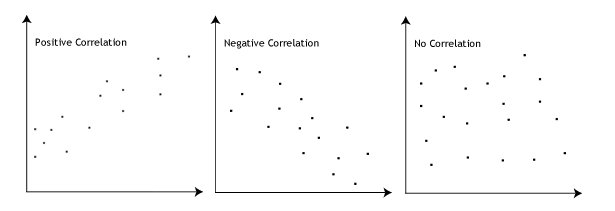
\includegraphics[width=0.7\linewidth]{Regre1}
%\end{figure}

\begin{itemize}
	\item The strength of the relation is represented in a numeric value known at the \textbf{correlation coefficient}. 
	\item This coefficient can take a value between -1 and 1. Additionally there are no units.
	
	\[ -1 \leq r \leq 1\]
	
	\item We can use the following graphic to help us interpret the correlation coefficient.
\end{itemize}
%\begin{figure}[h!]
%	\centering
%	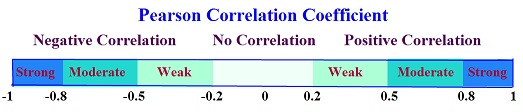
\includegraphics[width=0.9\linewidth]{pearson-correlation-coefficient-interpretation}
%\end{figure}
{
	
	\begin{framed}
		\begin{verbatim}
		> X
		[1] 104.40 104.14 104.84  99.34 104.13
		[6] 100.93 103.85  97.16  96.18 101.42
		> 
		> Y
		[1]  98.39 106.05 111.18  97.65 104.02
		[6] 100.18 106.20 101.87  92.49 101.41
		> 
		> cor(X,Y)
		[1] 0.7171676
		> 
		
		\end{verbatim}
	\end{framed}
}



The Pearson correlation coefficient is computed using the
following formula


\begin{itemize}
	\item $\sum x$ \item $\sum y$ \item $\sum xy$ \item $\sum x^2$
	\item $\sum y^2$
\end{itemize}

\begin{tabular}{|ccc|ccc|ccc|ccc|ccc|}
	\hline
	& X & & & Y & & &  $X^2$ & & &  $Y^2$ & & &  XY & \\
	& 1.0 & & & 10.6 & & &  1.00 & & &  36 & & &  90 & \\ \hline
	& 1.2 & & & 12.5 & & &  1.44 & & &  36 & & &  90 & \\ \hline
	& 1.6 & & & 14.7 & & &  2.56 & & &  36 & & &  90 & \\ \hline
	& 1.7 & & & 16.7 & & &  225 & & &  36 & & &  90 & \\ \hline
	& 1.8 & & & 18.7 & & &  225 & & &  36 & & &  90 & \\ \hline
	& 2.1 & & & 22.1 & & &  4.41 & & &  36 & & &  90 & \\ \hline
	
	
\end{tabular}

\[
r = { \; n \sum xy - \sum x \sum y   \; \over \left[\;\sqrt{n \sum (x^2) - (\sum x)^2} \;\right] \times  \left[ \;\sqrt{n \sum (y^2) - (\sum y)^2}\; \right]}
\]

\subsection*{Spearman and Kendall Correlation Coefficients}
\begin{itemize}
	\item Non-parametric statistics are statistics that do not require any special assumptions (i.e. Assumption of normality). 
	\item The \textbf{Spearman's rank-order} and \textbf{Kendall Tau} correlation coefficients are the \textbf{nonparametric} version of the Pearson product-moment correlation. 
	\item Both methods measure the strength of association between two \textbf{ranked} (ordinal) variables.
	\item  The coefficients are interpreted the same way as Pearson's Correlation Coefficient.
\end{itemize}

\begin{framed}
	\begin{verbatim}
	### Spearman Correlation Coefficient
	
	cor(X,Y, method="spearman")
	
	### Kendall Correlation Coefficient
	
	cor(X,Y, method="kendall")
	
	## [1] 0.6242424
	## [1] 0.5111111
	\end{verbatim}
\end{framed}

\subsection*{The Coefficient of Determination}
\begin{itemize}
	\item The coefficient of determination $R^2$ is the proportion of variability in a data set that is accounted for by the linear model. 
	\item Equivalently $R^2$ provides a measure of how well future outcomes are likely to be predicted by the model.
	
	\item For simple linear regression, it can be computed by squaring the correlation coefficient. It is not specifically defined that way. 
	\item This relationship is co-incidental when there are just two variables.
\end{itemize}
{
	
	\begin{framed}
		\begin{verbatim}
		> summary(lm(Y~X))
		
		Call:
		lm(formula = Y ~ X)
		....
		
		Coefficients:
		Estimate Std. Error t value
		(Intercept) -18.5506    41.4156  -0.448
		X             1.1855     0.4073   2.911
		Pr(>|t|)  
		(Intercept)   0.6661  
		X             0.0196 *
		....
		Residual standard error: 3.884 on 8 degrees of freedom
		Multiple R-squared:  0.5143,    Adjusted R-squared:  0.4536 
		F-statistic: 8.472 on 1 and 8 DF,  p-value: 0.01957
		
		\end{verbatim}
	\end{framed}
}




%-----------------------------------------------------------------------%

\subsection{Computing the Correlation Coefficient}

\[ \mbox{Cor(X,Y)} = \frac{\mbox{Cov}(X,Y)}{\sqrt{\mbox{Var}(X) \times \mbox{Var}(Y)}} \]

% http://easycalculation.com/statistics/learn-correlation.php








\subsubsection*{The Adjusted R-square value}
\noindent The adjusted R-square value is found on the summary output for a fitted model. It is called \textbf{\emph{adjusted}} because it takes into account the number of predictor variables being used. The law of parsimony states the simplest model that adequately explains the outcomes is the best. The candidate model with the higher adjusted R squared is considered preferable.

\subsubsection*{The Akaike Information Criterion}
\noindent The AIC is a model selection metric often used in statistics. It is computed using the R command
\texttt{\textbf{AIC()}}. The candidate model with the smallest AIC value is considered preferable.



\end{document}
	


%-------------------------------------------------%
